\chapter{Simulation}
\minitoc
\label{Cap:Simulation}

\section{Introduction}
\label{Cap:Simulation:Introduction}
The simulation of the MINER$\nu$A detector has multiple functions, such as background estimation, efficiency detector studies, simulation of reconstruction and the comparison of different  model with data. In this chapter, the different steps of the MINER$\nu$A experiment simulation are explained, including the beam simulation and a brief description of the models used by the simulators.

The simulation starts with the beam simulation, followed by the simulation of the neutrino interaction inside the MINER$\nu$A detector geometry. It proceeds with the simulation of the propagation of the resultant particles in the interaction with the detector; here the deposited energy, the particle track, and secondary particles are simulated. The last part of the simulation consists of a decalibration of the results from the preview stage in the way to simulate the same conditions of the real detector. In the end, it returns the simulated data in the same format as the raw data. In the following sections, the simulation steps are explained.

\section{Beam simulation}
\label{Cap:Simulation:BeamSimulation}

The neutrino flux simulation is performed in G4NuMI, based on GEANT 4 \cite{GEANT4}. In this stage, the production of hadrons, the focusing, and the secondary interactions of the hadrons with the different components of NuMI are simulated. It starts by giving the proton beam as input from the main injector and finishes with the neutrino beam. The simulation output is in the dk2nu format \cite{dk2nu}. The output includes information about the kinematics of the neutrino, the ancestors of the neutrino, paths through the magnetic field, and reinteractions of the mesons with the components of NuMI. This information is used by GENIE\cite{Genie} as input in the next stage of the simulation to simulate the neutrino interaction simulation in the detector.
 
After giving the as input the proton beam from the main injector, which corresponds to a 120 GeV kinetic energy with a Gaussian transverse profile distribution with $\sigma$ = 1.1 mm, continuing with the hadron production simulation. For hadron production, GEANT 4 uses the hadronic model FTFP\_BERT that is a combination of the FRITIOF \cite{PhysRevD.90.032001} and Bertini \cite{BERTINI1971670} \cite{GUTHRIE196829}cascade models. However, the reinteractions of the mesons with other components of NuMI are not well simulated because these interactions are modeled by non-perturbative QFT. The \textbf{Figure} \ref{fig:Simulation:Beam:HadIntperNu} shows the simulated number of hadronic interactions per neutrino as a function of the neutrino energy, from the figure the predominance of the $pC\rightarrow\pi X$ for the hadrons that produce the ME beam can be observed. 

\begin{figure}[!htb]
    \centering
    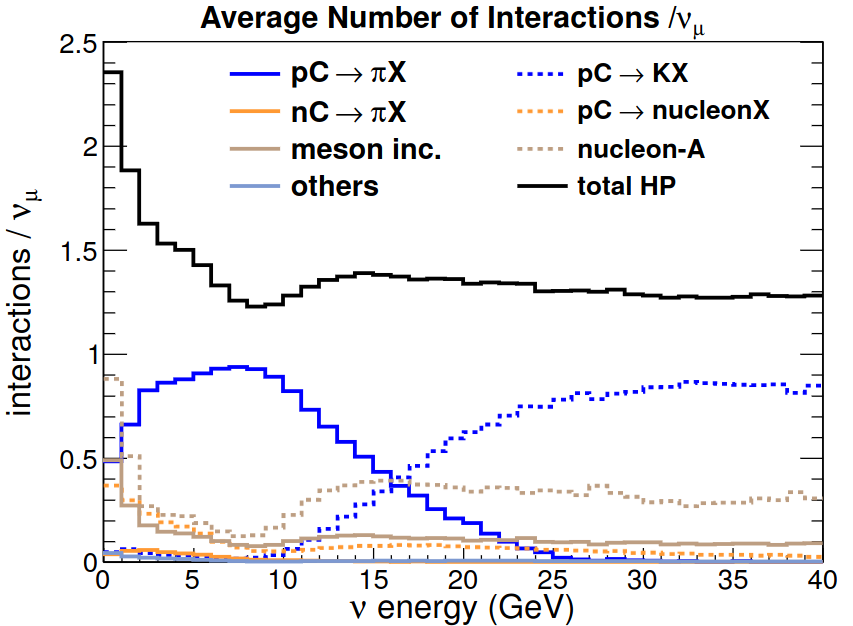
\includegraphics[scale=0.3]{Figures/Chapter3/HadronicInteractions.png}
    \caption{In this plot the simulated number of hadrons interactions per neutrino as function of the produced neutrino energy for the ME era are shown. Figure from \cite{LeoThesis}}
    \label{fig:Simulation:Beam:HadIntperNu}
\end{figure}

The current solution to constrain the models is to use the data obtained from NA49\cite{NA49}. In these studies \cite{NA49} the cross section results for charge pion production are shown, the interest in the production of the charge pions is because it is the dominant source of neutrinos in the neutrino beam. The pion yield, $f_{Data}$, from NA49 inelastic interactions is obtained by

\begin{equation}
    f_{Data}=E_\pi\frac{1}{\sigma_{inel}}\frac{d^3\sigma}{dp^3},
\end{equation}

where $E_\pi$ is the pion energy, $\sigma_{inel}$ is the total inelastic cross section, $p$ is the proton momentum. For the MC we have the equivalent relation. In the way to obtain the weight for the meson that produces the neutrino is 

\begin{equation}
    weight(x_F,p_T,p) = \frac{f_{Data}(x_F,p_T,p_0=158 GeV)}{f_{MC}(x_F,p_T,p_0=158 GeV)}s(x_F,p_T,p),
\end{equation}

where $x_F$ is the Feynman variable; $s$ is a factor scale 158 GeV to 120 GeV that corresponds to the main injector proton beam, calculated by FLUKA\cite{Fluka}; $p_T$ is the transverse momentum. 

 
\begin{figure}
    \centering
    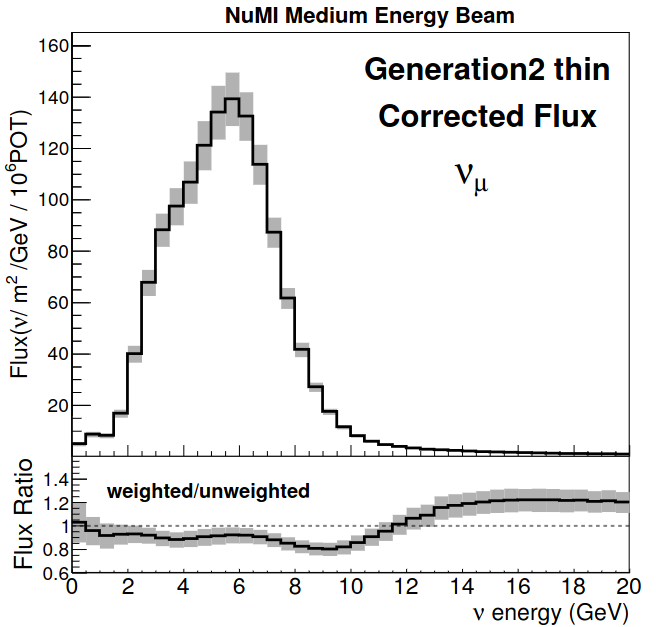
\includegraphics[scale=0.3]{Figures/Chapter3/FluxDistribution.png}
    \caption{Simulated neutrino flux distribution as function of the neutrino energy for the ME era. Figure from \cite{LeoThesis}}
    \label{fig:Simulation:Beam:FluxDistribution}
\end{figure}

\section{Interaction Simulation}
\label{Cap:Simulation:InteractionSimulation}

After simulating the neutrino beam, the next step is to simulate how these neutrinos interact with the MINER$\nu$A detector, this part of the simulation is performed using GENIE\cite{Genie}. GENIE brings information about the neutrino interaction, vertex kinematics, particle identities, the initial particles state, the ancestors of the particles, interactions inside of the nucleus and the final state particles kinematics. The results reported for this thesis include the MINER$\nu$A detector simulation using GENIE version 2.12.6. GENIE is described in more detail in the \textbf{Subsection} \ref{Cap:Simulation:GENIE}.

\subsection{GENIE}
\label{Cap:Simulation:GENIE}
GENIE is a ROOT-based neutrino event simulator in the C++ language. GENIE is capable to simulate neutrino interactions for a wide range of neutrino energy spectrum. This being very useful for a large number of experiments. The physics models used by GENIE can be categorized into nuclear physics models, cross-section models, and hadronization models.

\subsubsection{Nuclear Physics Model}
\label{Cap:Simulation:GENIE:NuclearPhysicsModel}

Depending on the energy of the neutrino, it can interact with matter through different mechanisms. At low energies, it interacts more with atoms and the nucleus as a whole, whereas at higher energies it interacts more deeply with the nucleus, potentially causing nuclear breakup. In addition, the products of the interaction may undergo further interactions with nuclear components before exiting the nucleus. The nuclear effects observed in an interaction strongly depend on the atom with which the neutrino interacts. Therefore, it is important to have accurate simulations of nuclear effects in various materials to enable better comparison with experimental data.

The GENIE simulator employs a Relativistic Fermi Gas (RFG) model to represent all processes within the nucleus \cite{RFGPhysRevC.80.065501}. It incorporates the Bodek and Ritchie modification for the high-momentum tail of nucleons \cite{BodekRichiePhysRevD.24.1400}. Additionally, the simulation incorporates Pauli blocking suppression for quasielastic and elastic scattering, which varies as a function of the atomic mass.

To simulate the Final State Interactions (FSI), GENIE uses external data measuring the hadron scattering in the nuclei and the effective cascade simulation implemented by the INTRANUKE module \cite{Genie}. 


\subsubsection{Cross Section Model}
\label{Cap:Simulation:GENIE:CrossSectionModel}

GENIE cross section models implemented for the Neutral Current (NC) and Charged Current (CC) interactions are the following:

\begin{itemize}
    \item \textbf{Quasi-Elastic Scattering:} The quasi-elastic interaction model implemented by GENIE based in the Llewellyn-Smith model \cite{LLEWELLYNSMITH1972261}. This model uses the general Lorentz-invariant form factors to model the hadronic weak current. The electromagnetic form factor parametrizations are found from electron scattering experiments results \cite{BRADFORD2006127}. The axial form factor shape is based in a conserved axial current hypothesis \cite{LLEWELLYNSMITH1972261}, giving to $F_A(Q^2)$ as a value to determine. The default axial mass is defined as $M_{A,CCQE}=0.99GeV$.
    
    \item \textbf{Elastic NC Scattering:} The model used to simulate the neutral current processes in GENIE is based in the Ahrens et al. model \cite{Ahrens:PhysRevD.35.785}, where the axial form factor only depends of an adjustable parameter $\eta$ that is set as $\eta=0.12$. 
    
    \item \textbf{Baryon Resonance Production:} This describe the CC and NC resonant neutrino interactions based in the Rein-Sehgal model \cite{REIN198179}. This model includes 16 of the 18 original resonances. The baryon resonance decays are characterized to produce charged or neutral pions. The GENIE model does not implement the interference between neighboring resonances. The lepton mass is only taken account the phase space boundaries but not for the cross section calculation. The resonant axial vector mass $M_{A,RES}$ = 1.12 GeV\cite{Kuzmin:2006dh} and the default vector mas value is $M_{v,RES}=0.84$ GeV. In a recent analysis the values for the $M_{A,RES}$ has been updated to 0.94 GeV. The simulation developed by MINERvA initially uses the original axial mass value, but it have been weighted in the order to use the updated value. In GENIE, the resonant events are simulated only for W < 1.7 GeV, above to this region the resonant and non-resonant interactions are modeled as DIS events. 
    
    \item \textbf{Coherent Neutrino-Nucleus Scattering:} GENIE simulates the NC and CC interaction channels. These are modeled by the Rein-Sehgal model \cite{REINcoh198329}. The model requires a small momentum transfer to the nucleus. It assumes a dipole dependence for non-zero $Q^2$ and axial mass of 1 GeV and then it uses the cross section results from pion scattering from protons and deuterium to normalize the value of the axial form factor at $Q^2=0$. 
    \item \textbf{Deep Inelastic Scattering:} GENIE simulates Deep Inelastic Scattering (DIS) events based in the Bodek and Yang model \cite{Bodek_2003} to describe scattering at $Q^2<1$ GeV. The Bodek-Yang model also produces resonant and non-resonant 1 pion events. To avoid double counting for $W<1.7$ GeV the Bodek-Yang model according to the cross section obtained in deuterium bubble chamber, the 1 pion and 2 pion production must be suppressed 43\%\cite{Rodrigues_2016}. 

    The AGKY model \cite{Yang_2009}is used to simulate the hadronization processes using the KNO \cite{KOBA1972317} scale for events with $W<2.3$ GeV while events with $W>3$ GeV are modeled by PYTHIA/JETSET \cite{PHYTIASJOSTRAND2001238}. for the middle range (2.3 GeV to 3 GeV) ans a linear scale of the two models is used to get a continuous distribution decreasing the interactions from AGKY and increasing the PYTHIA / JETSET as $W$ increase. 
    \item \textbf{Other Interaction Models:} GENIE also simulates other types of events such as Quasi-Elastic Charm Production\cite{CharmProd}, Deep-Inelatic Charm Production\cite{PhysRevD.50.3085}, Inclusive Inverse Muon Decay \cite{BARDIN1987839}, Neutrino-Electron Elastic Scattering \cite{William}.
    
\end{itemize}

\section{Detector Simulation}
\label{Cap:Simulation:DetectorSimulation}

This section describes how the propagation of FSI particles produced by neutrino interactions is simulated in the MINER$\nu$A detector. Geant4 \cite{GEANT4} is used to simulate the passage of these particles in the detector, taking into account the geometry and materials of the detector. After Geant4 simulates the passage of FSI particles in the detector, the next step is to recalibrate the energy reconstruction and transform this information into the same format as the raw data. 

\subsection{Geant4}
\label{Cap:Simulation:GEANT4}

To simulate the detector, it is necessary to include the whole geometry of the detector, the materials, the physical properties of the materials, and the physical processes that can be produced for the pass of the particles in the detector. 

Geant4 simulates the energy deposited by the particles, the elastic and inelastic scattering, and the tracking of the particles. Geant4 simulates by steps the pass of the particles. Each step has information of the four momenta of each particle and calculates the probability of how the particle interacts with the detector materials or if it will decay. 
The probabilities for strong elastic and inelastic scattering are given by the QGSP-BERT physics list \cite{1968Nuc} \cite{BERTINI1971670} \cite{Braun:1995pi} \cite{Alexander}. For the elastic electromagnetic, the EmStandard module is used. This module includes ionization, Coulomb scattering,  bremsstrahlung, photoelectric interactions, etc. The particle decays are modeled by the DecayPhysics module.

\section{Data overlay}
\label{Cap:Simulation:DataOverlay}
During data collection, the detector collects activity that comes from the neutrino interaction and from other sources. Activity not related to neutrino interactions is referred to as pileup, which can affect energy and tracking reconstruction. To incorporate these effects into the simulation, random data gates are overlayed onto simulated events.


\section{Readout simulation}
\label{Cap:Simulation:ReadoutSim}

The last step of the simulation consists in decalibrate the simulation made by Geant4 to raw ADC counts. The objective of this process is to apply the same reconstruction procedure to the data and MC. 

The steps to de-calibrate the simulation are listed here: 
\begin{enumerate}
    \item \textbf{Energy to photons:} It takes the deposited simulated energy from and estimates the light produced by the plastic scintillator strips.  
    \item \textbf{Light attenuation:} The light produced by the scintillator is attenuated for the scintillator, the Birks' law \cite{PhysRevD.98.030001} gives the attenuation of the light as function of the distance. The Birks' constant ($k_B =  0.0905 \pm 0.014 $ mm/MeV was obtained from the MINER$\nu$A test beam results\cite{minervacollaboration2015minerva}.)
    \item \textbf{From photons to energy:} The next stage is to determine the number of photo-electrons that are produced, to do it the de-calibrated energy from the previous step is divided MEU (see \ref{Cap:MnvExp:MnvDetector:Calibration:InSitu}). The attenuation light is added and the response correction are removed. 
    \item \textbf{Uncertainties of calibration Process:} To add the calibration process uncertainties the number of photons are multiplied by a random number from a Gaussian distribution centred in the 1. The standard deviation of the Gaussian is an estimate of the fractional uncertainty. 
    \item \textbf{PE in the PMT:} The next step is to pass the PE in to a raw ADC. The PMT simulation multiplies the signal as function of the gain obtained from the overlay, adds the cross talk and the electronic noise. With the known analog-to-digital response curves, the ADC counts are obtained. 
    \item \textbf{Timing decalibration:} It starts rounding the hit time to the closest 2.35 ns multiple. Then the offset of the time of each FEB and travel time for the photons is added to the hit time. To simulate the \textit{time-slewing} the hit time is smeared randomly by a distribution given the number of PE. 
\end{enumerate}

After making this de-calibration process, the simulated data is ready to be used by the same reconstruction algorithms that are used for data. 


\section{MINER$\nu$A Simulation Tuning}
\label{Cap:Simulation:MnvGENIETunes}

The simulation is not perfect, as it involves numerous effects, parameters, and model imperfections that can lead to inaccurate predictions of neutrino interactions. To address these imperfections, corrections can be introduced to the simulation by either incorporating new effects or adjusting existing models. This process involves rerunning the simulation to obtain an updated version or, alternatively, applying weights to the existing simulation. While the former option is computationally intensive, weighting is a more commonly employed approach because of its efficiency.

In MINER$\nu$A the weights correct the simulation products to the data results or theoretical modifications to the models. 

\subsection{Flux Reweight}
\label{Cap:Simulation:MnvGENIETunes:Flux}
The neutrino flux is simulated using G4NuMI. As detailed in Section \ref{Cap:Simulation:BeamSimulation}, the simulation includes all the steps to create the neutrino beam such as the hadron production, the focusing system, and the interaction of the hadrons with the NUMI components. Several corrections have been implemented, including adjustments to the geometry of the focusing horns. Additionally, various weights have been applied to enhance theoretical models, such as the Package to Predict the Flux (PPFX) \cite{LeoThesis}, and to account for effects like neutrino-electron elastic scattering and inverse muon decay.

The beam weights also depend of the playlist; it is because during the data collection small changes occur that can influence the resulting neutrino beam characteristics. 

\subsection{Muon Tracking Efficiency}
\label{Cap:Simulation:MnvGENIETunes:MinosEff}
In previous sections, It was mentioned that MINER$\nu$A used the MINOS ND as muon spectrometer. To use the MINOS detector as a muon spectrometer, it is necessary to match the muon track that exits the back of the MINER$\nu$A detector and enters the MINOS detector. The efficiency of this match is as a function of the muon momentum. The tracking efficiency was measured using the rock-muon data to be compared with the simulated tracking efficiency, obtaining an over-prediction of the efficiency. Therefore, all the matched tracks are corrected by a weight that depends on the muon momentum and the playlist. 

\begin{figure}
    \centering
    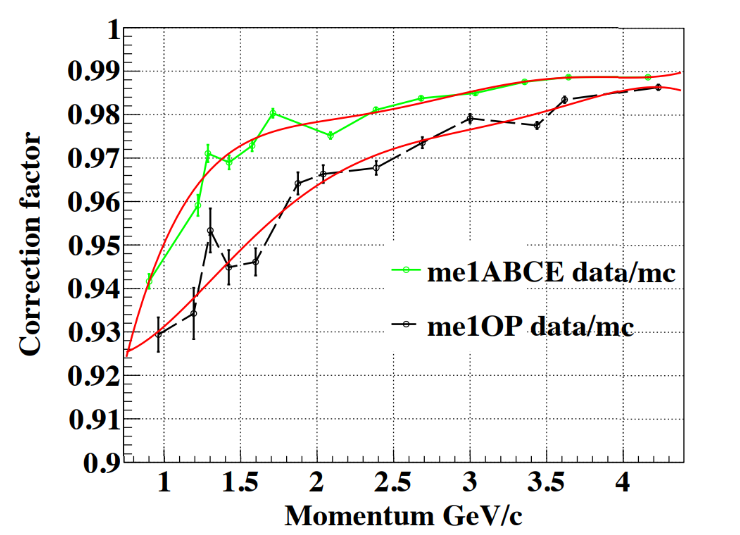
\includegraphics[scale=0.4]{Figures/Chapter3/MINOSEfficiencyWeight.png}
    \caption{Correction factor applied to the central value depending of the muon momentum for different playlists. Figure from \cite{MINOSEffWeight}}
    \label{fig:Chapter3:MINOSEfficiencyWeight}
\end{figure}

\subsection{Geant4 Weight}
\label{Cap:Simulation:MnvGENIETunes:Geant4Weight}
In the \textbf{Section} \ref{Cap:Simulation:GEANT4} is explained how Geant4 simulates the propagation of the FSI particles throughout the detector. MINER$\nu$A has developed weights that improve the simulation of the elastic and inelastic interactions during the propagation of particles. These weights adjust the production of charged pions, neutrons, and protons. 

The weight is obtained first by calculating the correction for the probability of no interaction, elastic and inelastic interactions as a function of the particle length track, the areal density and the improved and old cross section models. These weights are calculated by segments because the conditions of the materials change along the trajectory of the particles. The total event weight is obtained by multiplying all the weights for all the trajectories and the all the trajectories segments.  

The implementation of the weight calculation in small segments and not in infinitesimal steps is due to computational cost. However, it introduces imperfections to the weight. In order not to affect the number of neutrino events for this weight, the total event weight is normalized by a factor that keeps the number of neutrino events constant. These weights also depend on the type of particle. A detailed description of the calculation can be found here \cite{JeffreeThesis}.

In the case of the neutrons, the simulation is reweighted using the results cross section results from \cite{ElkinsNeutronsPhysRevD.100.052002}.

\subsection{MnvGENIE X.Y.Z}
\label{Cap:Simulation:MnvGENIETunes:MnvTunesXYZ}
The weights described in this section are related to modifications made to the theoretical model or corrections to the models that come from the data. The X, Y, and Z correspond to the different combinations that are made to modify the simulation. 
In the \textbf{Tables} \ref{tab:Simulation:MnvGENIETunes:X}, \ref{tab:Simulation:MnvGENIETunes:Y} and \ref{tab:Simulation:MnvGENIETunes:Z} the different versions are described with a description of each weight. 

\begin{table}[!htb]
    \centering
    \begin{tabular}{c|p{4.5in}}
        \textbf{X} & \textbf{Description} \\ \hline
        1 & This weight implements the effects of models that are not included in GENIE such as the random phase approximation (RPA) based in \cite{RPAPhysRevC.70.055503}\cite{RPAgran2017model}, Valencia 2p2h process \cite{2p2hPhysRevC.83.045501}\cite{2p2hGran_2013}\cite{2p2hRodrigues_2016} and the suppression of non-resonant pions\cite{Rodrigues_2016}. \\ \hline
        2 & This version includes the X=1 weights plus the pion low $Q^2$ suppression \cite{LowQ2PhysRevD.100.072005}.  \\ \hline
        3 & It uses the same weights as X = 1 but replaces the Valencia 2p2h model with SuSA 2p2h\cite{SuSAPhysRevC.38.1801} and the Bodek-Ritchie tail enhancement\cite{Alvarez_Ruso_2021}. It also removes 25 MeV from the $E_{avail}$ for pion events with protons in the final state. \\ \hline
        4 & It applies the same weights as X = 1 and the single pion production on deuterium correction. Changes the resonant pion production from the nominal value 1.12 GeV to 0.94 GeV, and modifies the CC resonant normalization from 1 to 1.15.  \\ 
    \end{tabular}
    \caption{Number specifies the version of the weight. To select the version only the weights that are specified must be applied, these are not cumulative. }
    \label{tab:Simulation:MnvGENIETunes:X}
\end{table}

\begin{table}[!htb]
    \centering
    \begin{tabular}{c|p{4.5in}}
        \textbf{Y} & \textbf{Description} \\ \hline
        1 & It normalizes the coherent production as function of the pion energy\cite{CoherentWeight}. \\ \hline
        2 & It normalizes the coherent production as function of the pion angle respect to the neutrino beam and the pion energy \cite{CoherentWeight}. \\ \hline
        3 & It uses the Y=2 weight and applies the low $Q^2$ suppression from the one pion production in the MINER$\nu$A targets and scintillator analysis \cite{AaronThesis}\cite{Bercellie.131.011801}. \\ \hline
        4 & This weight implements the z-expansion proposed by Mayer et. al. \cite{ZExpansionPhysRevD.93.113015} instead of the dipole shape for the axial form factor in quasi-elastic interactions.  \\ \hline
        5 & Substitute the Relativistic Fermi Gas (RFG) nuclear model with the NuWro Spectral Function (SF)\cite{GolanThesis}. \\ 
        
    \end{tabular}
    \caption{Number specifies the version of the weight. To select the version only the weights that are specified must be applied, these are not cumulative.}
    \label{tab:Simulation:MnvGENIETunes:Y}
\end{table}

\begin{table}[!htb]
    \centering
    \begin{tabular}{c|p{4.5in}}
        \textbf{Z} & \textbf{Description} \\ \hline
        1 & This weight corrects the bug in the FSI simulation in GENIE 2.12. These has an effect in the elastic FSI for pions and protons produced in the scintillator, other materials are not included. Correction based on \cite{harewood2019elastic}.  \\
    \end{tabular}
    \caption{Number specifies the version of the weight.}
    \label{tab:Simulation:MnvGENIETunes:Z}
\end{table}

This analysis implements two MnvGENIE Tunes, For the 1D analysis uses MnvGENIE v4.3.1 + Pion reweight, the pion reweight is explained in the section \ref{Cap:Simulation:MnvGENIETunes:PionReweight}. The 2D analysis uses the MnvGENIE v4.3.1 tune as nominal simulation.


\subsection{Pion Reweight }
\label{Cap:Simulation:MnvGENIETunes:PionReweight}

This weight is developed due an over prediction observed in the low $T_\pi$ region when the untracked pion reconstruction (explained in \ref{Cap:MnvExp:MnvDetector:DataReconstruction:Untrackedpions}) is used.

The method for obtaining this weight is the single value decomposition to give as input the migration matrix $M$ of the kinetic energy and the pion range. Let $M$ a $m\times n$ matrix to be factorized in the form $M=U\Sigma V^T$. Where $U$ ($m\times m$) and $v$ ($n\times n$) are singular unitary matrices, and $\Sigma$ is a $m\times n$ diagonal matrix where the numbers on the diagonal are positive real numbers. 

Next, the diagonal elements of the matrix $\Sigma$ are normalized with respect to the first value of the diagonal, obtaining the tolerance value for the regularization. The tolerance is selected for the value where $\chi^2$ is close to the freedom degrees, see \textbf{Figure} . The chosen value will be used to regularize the $\Sigma$ matrix.

\begin{figure}[!htb]
    \centering
    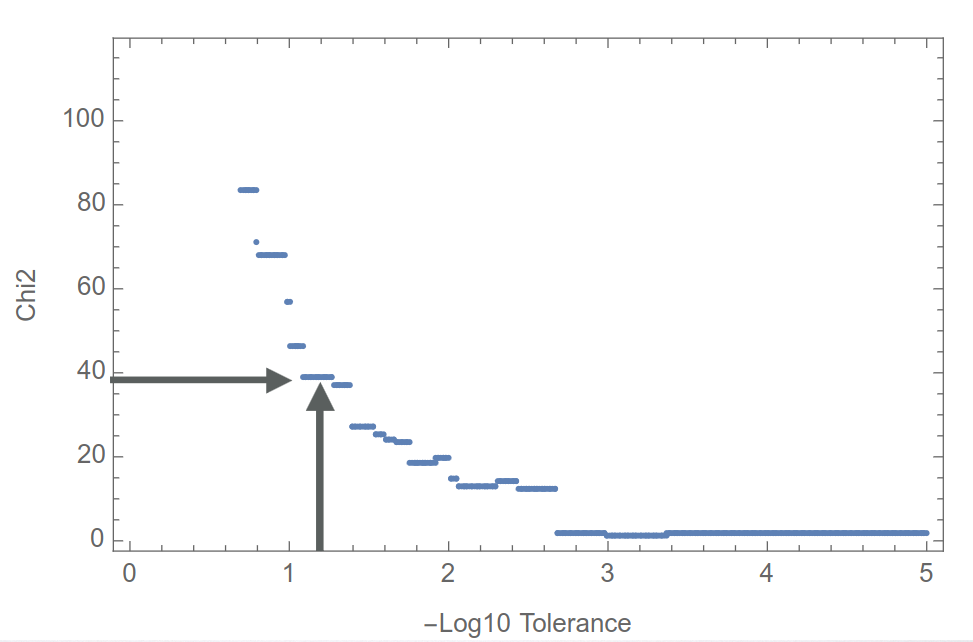
\includegraphics[scale=0.3]{Figures/Chapter3/ToleranceTpiweight.png}
    \caption{Tolerance vs $\chi^2$ for the unfolded spectrum. This the selected must give a reasonable $\chi^2$. Figure taken from \cite{PionReweight}.}
    \label{fig:Simulation:MnvGENIETunes:PionReweight:ToleranceTpiWeight}
\end{figure}

The inverse of the regularized matrix is used to obtain a pseudo inverse migration matrix as follows:

\begin{equation}
    M^+ = V\Sigma^{-1}_{reg} U^T
\end{equation}

where applying this to the reconstructed pion range for the data ($x_{Data}$) returns the new predicted value for the kinetic energy of the pion. 

\begin{equation}
    M^+ x_{Data} = y_{pred}
\end{equation}
 where $y_{pred}$ is the new distribution for the pion kinetic energy for a given tolerance value. The final weight is computed by taking the ratio between the MC $T_\pi$ distribution and $y_{\text{pred}}$. The weights obtained for various tolerance values are illustrated in \textbf{Figure} \ref{fig:Simulation:MnvGENIETunes:PionReweight:TpiWeight}. For the 1D analysis, the weight corresponding to a tolerance of 1.2 is selected. This choice is based on the smoother trend observed along this line.
 

\begin{figure}[!htb]
    \centering
    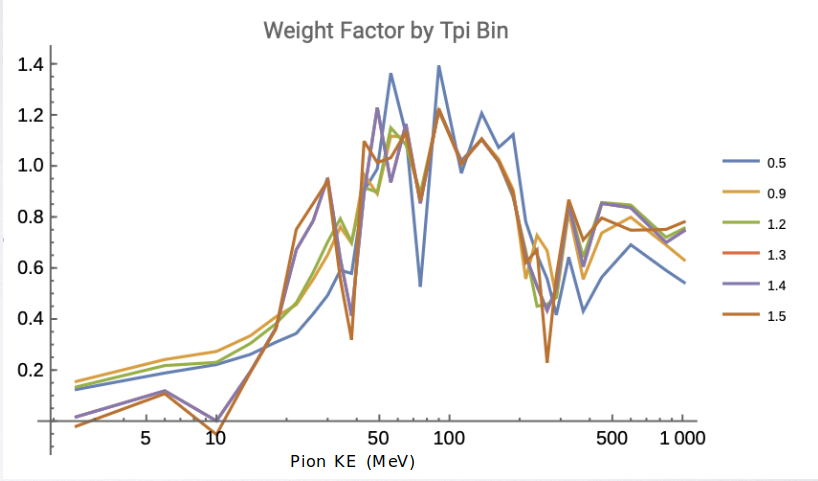
\includegraphics[scale=0.4]{Figures/Chapter3/TpiWeight.png}
    \caption{Value of the weights for each $T_\pi$ for different values of tolerance. Figure taken from \cite{PionReweight}.}
    \label{fig:Simulation:MnvGENIETunes:PionReweight:TpiWeight}
\end{figure}

